% Copyright (C) 2022-2023 Florin-Ioan Subțirică


\documentclass{article}

\usepackage{float}
\usepackage{tabularx}
\usepackage{siunitx}
\usepackage[a4paper, total={6in, 8in}]{geometry}
\usepackage[utf8]{inputenc}
\usepackage[english, romanian]{babel}
\usepackage[hidelinks]{hyperref}
\usepackage{indentfirst}
\usepackage[siunitx, RPvoltages]{circuitikz}
\usepackage{fancyhdr}
\usepackage{xspace}
\usepackage{amssymb}
\usepackage{layout}
\usepackage{lastpage}
\usepackage{titling}
\usepackage{leftidx}
\usepackage{array}
\usepackage{enumitem}
\usepackage{titletoc,tocloft}
\usepackage{xcolor}
\usepackage{amsmath}
\usepackage{nicefrac}
\usepackage{mathtools}
\usepackage{graphicx}
\graphicspath{ {./} }


% Configuring the \latex command with sane defaults
\newcommand{\latex}{\LaTeX\xspace}

% Configuring the margins and layout
\oddsidemargin  = 13pt
\headheight     = 12pt
\textheight     = 674pt
\marginparsep   = 10pt
\footskip       = 30pt
\hoffset        = 0pt
\paperwidth     = 597pt
\topmargin      = -23pt
\headsep        = 25pt
\textwidth      = 426pt
\marginparwidth = 50pt
\marginparpush  = 5pt
\voffset        = 0pt
\paperheight    = 845pt

% Removing default header & footer configuration
\fancyhf{}

% Configuring the header
\pagestyle{fancy}
\lhead[Fizică]{Fizică}
\rhead[Florin-Ioan Subțirică]{Florin-Ioan Subțirică}

% Configuring the footer
\fancyhf[FR]{Pagina \thepage\ din \pageref{LastPage}}

% Setting up links inside content table
\hypersetup {
    citecolor = black,
    filecolor = black,
    linkcolor = black,
    urlcolor  = black,
    colorlinks,
}

% Configuring the titlepage
\title          {Determinarea sarcinii specifice a electronului}
\author         {Florin-Ioan Subțirică \\ Seria CD, Grupa 322}
\date           {17.10.2022}
\predate{\centering}

\postdate{\vfill\emph{Facultatea de Automatică și Calculatoare}\hspace{2cm} \\
                \emph{Universitatea Politehnica București}     \hspace{2cm} \\
          \hfill\emph{2022 - 2023}\hfill}

% Configuring the table of contents
\setlength{\cftsubsecindent}{1cm}
\setlength{\cftsubsubsecindent}{2cm}
\dottedcontents{section}[1.5em]{}{1.3em}{.6em}



%%%%%%%%%%%%%%%%%%%%%%%%%%%%%%%%%%%%%%%%%%%%%%%%%%%%%%%%%%%%%%%%%%%%%%%%%%%%%%%


\begin{document}

% Project title
\maketitle
\thispagestyle{empty} % Remove page number
\pagebreak

% Table of contents
\tableofcontents
\thispagestyle{empty}
\pagebreak

% Introduction
\section        {Scopul lucrării}

    \makebox[1cm]{} Studiul mișcării electronilor într-un câmp magnetic uniform și determinarea
    valorii sarcinii specifice a electronului.

\section        {Principiul lucrării}

    \makebox[1cm]{} Electronii emiși de un filament metalic încălzit, accelerați de un câmp electric,
    pătrund într-o regiune unde este un câmp magnetic uniform. Datorită forței Lorentz,
    traiectoria electronilor este elicoidală, când unghiul dintre viteza electronilor
    și direcția câmpului magnetic este în intervalul (0, $\pi$/2), respectiv circulară,
    când unghiul este $\pi$/2 (viteza electronilor perpendiculară pe direcția câmpului magnetic).
    Valoarea sarcinii specifice se obține din valorile tensiunii de accelerare, inducției magnetice
    și razei orbitei circulare a electronului.

\section        {Teoria lucrării}

    \makebox[1cm]{} Dacă un electron (în repaus) de masă \textit{m} și sarcină \textit{e}
    este accelerat de o diferență de potențial \textit{U}, el va căpăta 
    energia cinetică \textit{${E}{_c}$}:
\begin{equation}
    {E}{_c} = \frac{1}{2}mv^2 = eU
\end{equation}
\raggedright
    unde \textit{v} este viteza electronului.

    \makebox[1.5cm]{} Dacă electronul, care are viteza $\vec{v}$, se mișcă într-o regiune unde este
    un câmp magnetic de inducție $\vec{B}$ /1/, asupra acestuia va acționa forța Lorentz /2/:
\begin{equation}
    \vec{F} = -e\vec{v}\times\vec{B}
\end{equation}
    \makebox[1.5cm]{} Dacă câmpul magnetic este uniform, așa cum (aproape) este cazul într-o configurație
    de tip Helmholtz /3,4/ a două bobine, traiectoria electronilor este elicoidală în
    lungul linilor de câmp magnetic. Când viteza electronilor este perpendiculară pe
    direcţia câmpului magnetic, traiectoria devine circulară (cum câmpul magnetic
    nu schimbă mărimea vitezei, ci doar direcţia acesteia, mişcarea este circulară uniformă).
    Forţa Lorentz este o forţă centripetă, astfel că legea a doua a lui Newton se scrie:
\begin{equation}
    \frac{mv^2}{r} = evB
\end{equation}
    unde r este raza traiectoriei circulare.

    Astfel, ecuaţiile \textbf{(1)}+\textbf{(3)} conduc la următoarea expresie pentru sarcina specifică:
\begin{equation}
    \frac{e}{m} = \frac{2U}{B^2r^2}
\end{equation}
    Inducția câmpului magnetic produs de 2 bobine Helmholtz în centrul sistemului este:
\begin{equation}
    B = (\frac{4}{5})^\frac{3}{2}{\mu}{_0}n\frac{I}{R}
\end{equation}
    unde ${\mu}{_0}$ este constanta magnetică a vidului /5/ ${\mu}{_0} = 4\pi \cdot 10^{-7}NA^{-2}$, n
    este numărul de spire din fiecare bobină iar R este raza bobinelor (pentru această experienţă
    n = 154 şi R = 0,2m); pe axa bobinelor, câmpul magnetic se obţine din legea Biot-Savart-Laplace,
    iar configuraţia Helmholtz implică că distanţa dintre bobine este egală cu raza bobinelor,
    şi în acest caz câmpul magnetic este aproape uniform în spaţiul dintre bobine, şi este dat
    de formula \textbf{(5)}. Din ecuaţiile \textbf{(4)} şi \textbf{(5)}, se obţine:
\begin{equation}
    I^2 = \frac{125}{32}\frac{R^2}{{{\mu}{_0}}^2n^2}\frac{1}{\frac{e}{m}}\frac{U}{r^2}
\end{equation}    

\begin{equation}
    \frac{e}{m} = \frac{125}{32}\frac{R^2}{{{\mu}{_0}}^2n^2}\frac{U}{r^2I^2} \newline
\end{equation}

\raggedright
\section        {Dispozitivul experimental}

\makebox[1.5cm]{} Dispozitivul experimental pentru determinarea sarcinii specifice
a electronului este prezentat în Fig. 1 şi cuprinde:

    - un tub din sticlă, umplut cu neon la joasă presiune, în care se găseşte tunul electronic;\newline
    - o pereche de bobine Helmholtz;\newline
    - sursa de alimentare a bobinelor (max. 18$\si{\volt}$/5$\si{\ampere}$; se foloseşte la o
    putere de 2$\si{\watt}$);\newline
    - sursa de alimentare a filamentului tunului de electroni (6,3$\si{\volt}$/2$\si{\ampere}$),
    a grilei de selecţie şi focalizare a electronilor (0-50$\si{\volt}$) şi a electrozilor
    de accelerare a electronilor (0-300$\si{\volt}$);\newline
    - ampermetru (scala de 10$\si{\ampere}$) pentru măsurarea curentului prin bobine; \newline
    - voltmetru (scala de 600$\si{\volt}$) pentru măsurarea tensiunii de grilă şi a
    tensiunii de accelerare;\newline
    - cabluri de legătură, de diverse lungimi şi culori.\newline

\makebox[1.5cm]{} Schemele electrice pentru alimentarea bobinelor Helmholtz (care produc
    câmpul magnetic aproape uniform în spaţiul dintre bobine) şi a tunului electronic sunt
    prezentate in Fig. 2 şi Fig. 3. 

\begin{figure}[H]
    \centering
    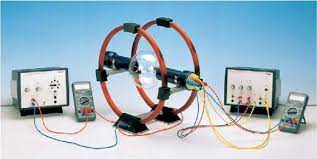
\includegraphics[scale = 0.6]{Aranjamentul experimental.jpeg}
    \caption{Aranjamentul experimental pentru determinarea sarcinii specifice a electronului}
\end{figure}

\begin{figure}[H]
    \centering
    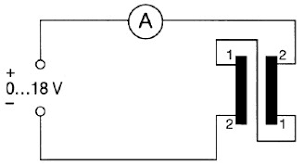
\includegraphics[scale = 0.6]{Alimentarea bobinelor Helmholtz .png}
    \caption{Alimentarea bobinelor Helmholtz}
\end{figure}

\begin{figure}[H]
    \centering
    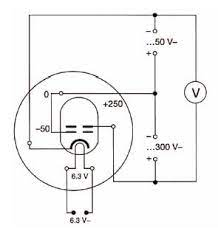
\includegraphics[scale = 0.6]{Alimentarea tunului electronic.jpeg}
    \caption{Alimentarea tunului electronic, din tubul cu neon la joasă presiune}
\end{figure}

\section        {Modul de lucru și prelucrarea datelor experimentale}

\makebox[1.2cm]{} Primul pas, înainte de alimentarea electrică a aparatului, am verificat toate conexiunile,
după care am setat potențiometrele pe minim (pentru a evita arderea aparatului), iar mai apoi
am pornit cele două multimetre.

\makebox[1.2cm]{} Am setat sursa de alimentare a bobinelor la 2W și limitatorul de intensitate
a curentului la 3A, pentru a evita supraîncălzirea prematură, iar apoi am mărit
tensiunea sursei de alimentare a tunului electronic la 20V (tensiunea de grilă).

\makebox[1.2cm]{} O dată cu creșterea tensiunii de accelerare până la 120V (multimetrul indicând 140V, datorită
faptului că 20V cad pe grilă - tensiunea de grilă), deja se putea observa traiectoria rectilinie a electronilor prin
tub, vizibilă datorită ciocnirii electronilor cu atomii de neon din tub.

\makebox[1.2cm]{} Mărind tensiunea sursei bobinelor, crește inducția câmpului magnetic, care este proporțională
cu forța Lorenz ce acționează asupra electronilor, deci astfel traiectoria lor se curbează și
devine circulară, raza acesteia scăzând odată cu mărirea tensiunii.(Fig.4)

\begin{figure}[H]
    \centering
    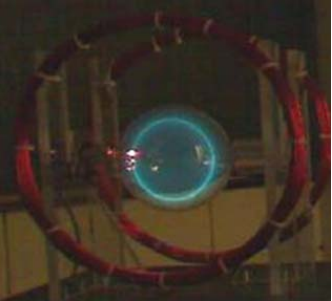
\includegraphics[scale = 0.62]{vedere a bobinelor helmholtz.png}
    \caption{Vedere a bobinelor Helmholtz şi a traiectoriei electronilor}
\end{figure}

\begin{figure}[H]
    \centering
    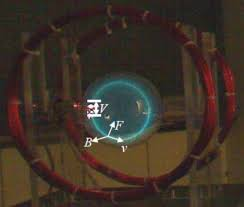
\includegraphics[scale = 0.8]{tens acc U, ind mag.jpeg}
    \caption{Indicarea tensiunii acceleratoare U, a inducției magnetice, a vitezei 
         tangențiale la traiectoria circulară, și a forței Lorenz centripete}
\end{figure} 

\centering
    \break
    Tabelul 1. Valorile curentului prin bobinele Helmholtz pentru o tensiune de grilă de 20\si{\volt},
    tensiunea de accelerare de 160 \si{\volt} și raza de 4 cm.

\begin{table}[H]
    \begin{tabular}{|c|c|c|c|c|c|c|c|c|c|c|c|}
    \hline
    \begin{tabular}[c]{@{}c@{}}r\\ ($\si{\cm}$)\end{tabular} & \begin{tabular}[c]{@{}c@{}}U\\ ($\si{\volt}$)\end{tabular} & \begin{tabular}[c]{@{}c@{}}${I}{_1}$\\ ($\si{\ampere}$)\end{tabular} & \begin{tabular}[c]{@{}c@{}}${I}{_2}$\\ ($\si{\ampere}$)\end{tabular} & \begin{tabular}[c]{@{}c@{}}${I}{_3}$\\ ($\si{\ampere}$)\end{tabular} & \begin{tabular}[c]{@{}c@{}}${I}{_4}$\\ ($\si{\ampere}$)\end{tabular} & \begin{tabular}[c]{@{}c@{}}${I}{_5}$\\ ($\si{\ampere}$)\end{tabular} & \begin{tabular}[c]{@{}c@{}}${I}{_m}$\\ ($\si{\ampere}$)\end{tabular} & \begin{tabular}[c]{@{}c@{}}${\sigma}{_{I}{_m}}$\\ ($\si{\ampere}$)\end{tabular} & ${\epsilon}{_{I}{_m}}$ & \begin{tabular}[c]{@{}c@{}}B\\ ($\si{\tesla}$)\end{tabular} & \begin{tabular}[c]{@{}c@{}}\textless{}e/m\textgreater\\ ($\si{\coulomb}/\si{\kg}$)\end{tabular} \\ \hline
    4                                                        & 160                                                        & 1.613                                                                & 1.610                                                                & 1.606                                                                & 1.616                                                                & 1.615                                                                & 1.612                                                                & 1.8166e-03                                                                      & 1.1269e-03             & 1.1161e-03                                                  & 1.6056e+11                                                                         \\ \hline
    \end{tabular}
    \end{table}

\begin{equation*}
    unde \ {I}{_m} = \frac{\sum_{k=1}^{N} {I}{_m}}{N}, \ 
    {\sigma}{_{I}{_m}} = \sqrt{\frac{\sum_{k=1}^{N} ({I}{_k}-{I}{_m})^2}{N(N-1)}}, \
    {\epsilon}{_{I}{_m}} = \frac{{\sigma}{_{I}{_m}}}{{I}{_m}}, \ N = 5.
\end{equation*}
\raggedright
Știind că :
\begin{equation*}
    {\sigma}{_{\langle\frac{e}{m}\rangle}} = {\epsilon}{_{\langle\frac{e}{m}\rangle}} \cdot {\langle\frac{e}{m}\rangle} = (3.6187 \cdot 10^8) \ \si{\coulomb}/\si{\kg}, unde
    \ {\epsilon}{_{\langle\frac{e}{m}\rangle}} = 2{\epsilon}{_{I}{_m}} = 2.2538 \cdot 10^{-3}
\end{equation*}
prin urmare, rezultă că ne putem aștepta ca măsurătorile ulterioare să aibă o eroare foarte mică.

\hfill

\makebox[1.2cm]{} Următorul pas a fost să efectuăm măsurători și pentru alte raze și tensiuni de 
accelerare, calculând valorile sarcinii specifice în mod automat cu ajutorul unor scripturi
scrise în Octave. \newline

\centering
    Tabelul 2. Valorile curentului prin bobinele Helmholtz pentru o tensiune de grilă
    de 20 $\si{\volt}$, diverse tensiuni de accelerare şi diverse raze ale traiectoriilor electronilor.

\begin{table}[H]
    \begin{tabular}{|c|cc|cc|cc|cc|}
    \hline
                                                    & \multicolumn{2}{c|}{r = 5 cm}                                                                                               & \multicolumn{2}{c|}{r = 4 cm}                                                                                               & \multicolumn{2}{c|}{r = 3 cm}                                                                                               & \multicolumn{2}{c|}{r = 2 cm}                                                                                               \\ \hline
    \begin{tabular}[c]{@{}c@{}}U\\ (V)\end{tabular} & \multicolumn{1}{c|}{\begin{tabular}[c]{@{}c@{}}I\\ (A)\end{tabular}} & \begin{tabular}[c]{@{}c@{}}e/m\\ (C/kg)\end{tabular} & \multicolumn{1}{c|}{\begin{tabular}[c]{@{}c@{}}I\\ (A)\end{tabular}} & \begin{tabular}[c]{@{}c@{}}e/m\\ (C/kg)\end{tabular} & \multicolumn{1}{c|}{\begin{tabular}[c]{@{}c@{}}I\\ (A)\end{tabular}} & \begin{tabular}[c]{@{}c@{}}e/m\\ (C/kg)\end{tabular} & \multicolumn{1}{c|}{\begin{tabular}[c]{@{}c@{}}I\\ (A)\end{tabular}} & \begin{tabular}[c]{@{}c@{}}e/m\\ (C/kg)\end{tabular} \\ \hline
    120                                             & \multicolumn{1}{c|}{{\color[HTML]{FE0000} 0.004}}                    & -                                                    & \multicolumn{1}{c|}{\color[HTML]{FE0000} 0.173}                      & -                                                    & \multicolumn{1}{c|}{\color[HTML]{FE0000} 1.056}                      & -                                                    & \multicolumn{1}{c|}{2.861}                                           & 1.5291e+11                                           \\ \hline
    140                                             & \multicolumn{1}{c|}{1.204}                                           & 1.6117e+11                                           & \multicolumn{1}{c|}{1.489}                                           & 1.6466e+11                                           & \multicolumn{1}{c|}{1.997}                                           & 1.6274e+11                                           & \multicolumn{1}{c|}{3.143}                                           & 1.4782e+11                                           \\ \hline
    160                                             & \multicolumn{1}{c|}{1.295}                                           & 1.5922e+11                                           & \multicolumn{1}{c|}{1.611}                                           & 1.6076e+11                                           & \multicolumn{1}{c|}{2.180}                                           & 1.5607e+11                                           & \multicolumn{1}{c|}{3.349}                                           & 1.4880e+11                                           \\ \hline
    180                                             & \multicolumn{1}{c|}{1.364}                                           & 1.6146e+11                                           & \multicolumn{1}{c|}{1.725}                                           & 1.5774e+11                                           & \multicolumn{1}{c|}{2.328}                                           & 1.5397e+11                                           & \multicolumn{1}{c|}{3.613}                                           & 1.4383e+11                                           \\ \hline
    200                                             & \multicolumn{1}{c|}{1.455}                                           & 1.5766e+11                                           & \multicolumn{1}{c|}{1.807}                                           & 1.5972e+11                                           & \multicolumn{1}{c|}{2.428}                                           & 1.5727e+11                                           & \multicolumn{1}{c|}{3.820}                                           & 1.4296e+11                                           \\ \hline
    220                                             & \multicolumn{1}{c|}{1.503}                                           & 1.6253e+11                                           & \multicolumn{1}{c|}{1.895}                                           & 1.5975e+11                                           & \multicolumn{1}{c|}{2.569}                                           & 1.5453e+11                                           & \multicolumn{1}{c|}{3.905}                                           & 1.5048e+11                                           \\ \hline
    240                                             & \multicolumn{1}{c|}{1.603}                                           & 1.5587e+11                                           & \multicolumn{1}{c|}{1.975}                                           & 1.6044e+11                                           & \multicolumn{1}{c|}{2.625}                                           & 1.6146e+11                                           & \multicolumn{1}{c|}{4.010}                                           & 1.5568e+11                                           \\ \hline
    260                                             & \multicolumn{1}{c|}{1.646}                                           & 1.6015e+11                                           & \multicolumn{1}{c|}{2.040}                                           & 1.6291e+11                                           & \multicolumn{1}{c|}{2.783}                                           & 1.5562e+11                                           & \multicolumn{1}{c|}{\color[HTML]{FE0000} $\rangle$5}                 & -                                                    \\ \hline
    280                                             & \multicolumn{1}{c|}{1.704}                                           & 1.6093e+11                                           & \multicolumn{1}{c|}{2.115}                                           & 1.6322e+11                                           & \multicolumn{1}{c|}{2.895}                                           & 1.5487e+11                                           & \multicolumn{1}{c|}{\color[HTML]{FE0000} $\rangle$5}                 & -                                                    \\ \hline
    300                                             & \multicolumn{1}{c|}{1.759}                                           & 1.6181e+11                                           & \multicolumn{1}{c|}{2.215}                                           & 1.5945e+11                                           & \multicolumn{1}{c|}{2.957}                                           & 1.5905e+11                                           & \multicolumn{1}{c|}{\color[HTML]{FE0000} $\rangle$5}                 & -                                                    \\ \hline
    \end{tabular}
    \end{table}
\raggedright

\makebox[1.2cm]{} Unele măsurători au fost mult prea departe de adevăr, iar altele nu au putut fi deloc măsurate din cauza limitărilor de intensitate, prin urmare
    le-am pus cu roșu în tabel. Astfel, nu putem observa traiectoria electronilor la valori mici de intensitate și tensiune,
    iar la valori prea mari există riscul de supraîncălzire, chiar scurtcircuitate a aparatului.
\begin{equation*}
    {\langle\frac{e}{m}\rangle} = \frac{\sum_{k=1}^{K} {(e/m)}{_k}}{K} = (1.5728 \cdot 10^{11}) \ \si{\coulomb}/\si{\kg} $$\\$$
    {\sigma}{_{e/m}} = \sqrt{\frac{\sum_{k=1}^{K} ({(e/m)}{_k}-{\langle e/m \rangle})^2}{K(K-1)}} = (9.4057 \cdot 10^8) \ \si{\coulomb}/\si{\kg} $$\\$$
    {\epsilon}{_{\langle e/m \rangle}} = \frac{{\sigma}{_{\langle e/m \rangle}}}{\langle e/m \rangle} = 5.9803 \cdot 10^{-3}
\end{equation*} 
\raggedright iar K este numărul total de valori obținute (34). \newline

\makebox[1.5cm]{} Cu aceste date experimentale, am realizat reprezentarea grafică a
dependenței pătratului intensităţii curentului prin bobine în funcţie de raportul $U/r^2$.
    Conform formulei \textbf{(6)}, această dependență este o dreaptă care trece prin origine și are panta:
\begin{equation*}
    \alpha = \frac{125}{32}\frac{R^2}{{{\mu}{_0}}^2n^2}\frac{1}{\frac{e}{m}} = 2.7105 \cdot 10^{-5}
\end{equation*} de unde se obține valoarea sarcinii specifice:
\begin{equation*}
    \frac{e}{m} = \frac{125}{32}\frac{R^2}{{{\mu}{_0}}^2n^2}\frac{1}{\alpha} = 1.5393 \cdot 10^{11}(C/kg)
\end{equation*}
, valoare destul de apropiată de cea obținută prin calcule.

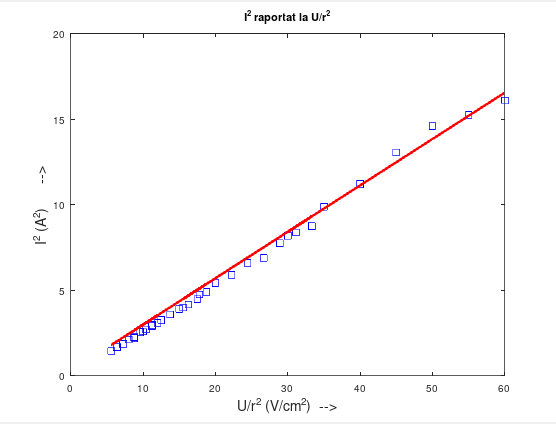
\includegraphics[scale = 0.7]{plot.png}
$$\emph{\footnotesize Dependența pătratului intensităţii curentului prin bobine în funcţie de raportul $U/r^2$ } $$

\section{Anexă}
\space\space\space\space \href{https://ctipub-my.sharepoint.com/:f:/g/personal/florin_subtirica_stud_acs_upb_ro/Eq0TbKFmnjhAoszjx_vnN18Bn3oi9FP3BmvfzAQFApd__Q?e=SbfAlY}{Referat} \newline

\begin{thebibliography}{10}

    $1. \space\space\space\space \href{https://en.wikipedia.org/wiki/Magnetic_field}{https://en.wikipedia.org/wiki/Magnetic_field} \newline
    2. \space\space\space\space \href{https://en.wikipedia.org/wiki/Lorentz_force}{https://en.wikipedia.org/wiki/Lorentz_force}  \newline
    3. \space\space\space\space \href{https://en.wikipedia.org/wiki/Helmholtz_coil}{https://en.wikipedia.org/wiki/Helmholtz_coil} \newline
    4. \space\space\space\space \href{http://physicsx.pr.erau.edu/HelmholtzCoils/}{http://physicsx.pr.erau.edu/HelmholtzCoils/}  \newline
    5. \space\space\space\space \href{http://physics.nist.gov/cgi-bin/cuu/Value?mu0}{http://physics.nist.gov/cgi-bin/cuu/Value?mu0}    \newline
    6. \space\space\space\space \href{http://physics.nist.gov/cgi-bin/cuu/Value?esme}{http://physics.nist.gov/cgi-bin/cuu/Value?esme}$

\end{thebibliography}
        
    \addcontentsline{toc}{section}{7 Bibliografie}

\end{document}

%%%%%%%%%%%%%%%%%%%%%%%%%%%%%%%%%%%%%%%%%%%%%%%%%%%%%%%%%%%%%%%%%%%%%%%%%%%%%%%
